\begin{figure}[tbp]
\centering
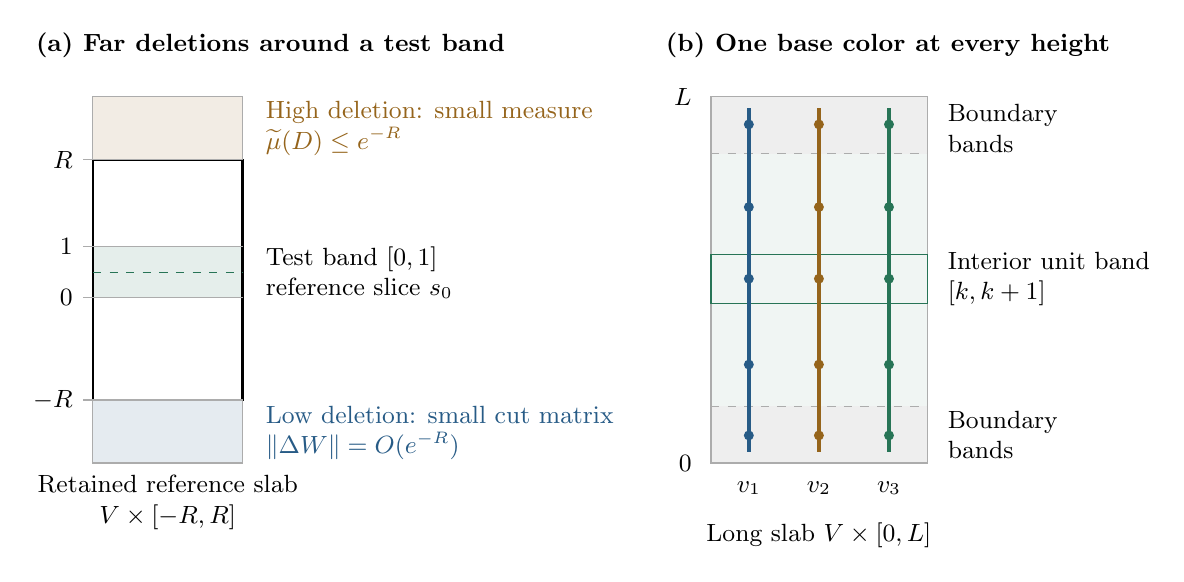
\begin{tikzpicture}[x=1cm,y=1cm,font=\small,
  every node/.style={inner sep=2pt},
  heightline/.style={gray!65,thin},
  fiber/.style={very thick}]
  \definecolor{mahblue}{RGB}{39,91,134}
  \definecolor{mahgold}{RGB}{149,100,27}
  \definecolor{mahgreen}{RGB}{39,116,86}

  \node[anchor=west,font=\small\bfseries] at (0,5.7)
    {(a) Far deletions around a test band};
  \fill[mahgold!12] (.8,4.25) rectangle (2.7,5.05);
  \fill[mahblue!12] (.8,.4) rectangle (2.7,1.2);
  \fill[mahgreen!12] (.8,2.5) rectangle (2.7,3.15);
  \draw[heightline] (.8,.4) rectangle (2.7,5.05);
  \draw[thick] (.8,1.2) rectangle (2.7,4.25);
  \foreach \y/\t in {1.2/{-R},2.5/{0},3.15/{1},4.25/{R}} {
    \draw[heightline] (.68,\y)--(2.7,\y);
    \node[anchor=east] at (.62,\y) {$\t$};
  }
  \draw[dashed,mahgreen] (.8,2.82)--(2.7,2.82);
  \node[anchor=west,align=left,text=mahgold] at (2.92,4.65)
    {High deletion: small measure\\$\widetilde\mu(D)\leq e^{-R}$};
  \node[anchor=west,align=left] at (2.92,2.82)
    {Test band $[0,1]$\\reference slice $s_0$};
  \node[anchor=west,align=left,text=mahblue] at (2.92,.78)
    {Low deletion: small cut matrix\\$\|\Delta W\|=O(e^{-R})$};
  \node[align=center] at (1.75,-.1)
    {Retained reference slab\\$V\times[-R,R]$};

  \node[anchor=west,font=\small\bfseries] at (8,5.7)
    {(b) One base color at every height};
  \fill[gray!13] (8.65,.4) rectangle (11.4,1.12);
  \fill[gray!13] (8.65,4.33) rectangle (11.4,5.05);
  \fill[mahgreen!7] (8.65,1.12) rectangle (11.4,4.33);
  \draw[heightline] (8.65,.4) rectangle (11.4,5.05);
  \draw[heightline,dashed] (8.65,1.12)--(11.4,1.12);
  \draw[heightline,dashed] (8.65,4.33)--(11.4,4.33);
  \draw[mahgreen] (8.65,2.43) rectangle (11.4,3.05);
  \foreach \x/\c in {9.13/mahblue,10.02/mahgold,10.91/mahgreen} {
    \draw[fiber,\c] (\x,.54)--(\x,4.91);
    \foreach \y in {.75,1.65,2.74,3.65,4.7}
      \fill[\c] (\x,\y) circle (1.8pt);
  }
  \node[anchor=east] at (8.48,.4) {$0$};
  \node[anchor=east] at (8.48,5.05) {$L$};
  \node[anchor=west,align=left] at (11.58,4.65) {Boundary\\bands};
  \node[anchor=west,align=left] at (11.58,2.74)
    {Interior unit band\\$[k,k+1]$};
  \node[anchor=west,align=left] at (11.58,.76) {Boundary\\bands};
  \node at (9.13,.08) {$v_1$};
  \node at (10.02,.08) {$v_2$};
  \node at (10.91,.08) {$v_3$};
  \node[align=center] at (10.02,-.52)
    {Long slab $V\times[0,L]$};
\end{tikzpicture}
\caption{Height geometry behind Lemmas~\ref{lem:far-deletion}
and~\ref{lem:coherent-choice} (not to scale). High and low deletions
are controlled by different estimates. A color selected on the
reference slice is used at every height above the same base vertex.
Translated interior unit bands compare with the reference slab in
integrated normalized data; the boundary bands have total length at
most $2R+2$. The colored vertical lines are base fibers
$\{v\}\times[0,L]$, not lifted relation orbits.}
\label{fig:maharam}
\end{figure}
